\documentclass[xcolor=table, aspectratio=169]{beamer}

% !TEX engine = pdflatex
%\usepackage{arev}
\usepackage{amsmath,amssymb,amscd}
\usepackage{dsfont}
\usepackage{mathrsfs}
\usepackage{yfonts}
\usepackage{bm}
\usepackage{graphicx}
\usepackage{tabularx}
\usepackage{animate}
\usepackage{listings}
%\usepackage{mathtools}
%\usepackage{ifthen}

%\usepackage{xeCJK}
%\usepackage{fontspec}
%\newfontfamily\cjkfont{PingFang SC}
%\setCJKmainfont{PingFang SC}
\newcolumntype{x}{>{\centering\arraybackslash}X}
\renewcommand{\arraystretch}{1.5}
\newcommand{\uone}{\mathrm U(1)}
%\newcommand{\uone}{\mathbb R/\mathbb Z}
\DeclareMathOperator{\img}{img}
\DeclareMathOperator{\hhom}{Hom}
\DeclareMathOperator{\id}{id}
\usepackage{tikz}
	\usetikzlibrary{calc}
	\usetikzlibrary{arrows,shapes, positioning, matrix}
	\usetikzlibrary{decorations.markings}
	\tikzset{>=stealth}
	\tikzstyle arrowstyle=[scale=1]
	\tikzstyle directed=[postaction={decorate,decoration={markings,
 	   mark=at position .15 with {\arrow[arrowstyle]{stealth}}}}]
\tikzstyle string=[thick,postaction={decorate,decoration={markings,
    mark=at position .55 with {\arrow[arrowstyle]{stealth}}}}]
\tikzstyle dual_string=[dashed,postaction={decorate,decoration={markings,
    mark=at position .55 with {\arrow[arrowstyle]{stealth}}}}]

\tikzstyle dw=[thick,postaction={decorate,decoration={markings,
    mark=at position 1 with {\arrow[arrowstyle]{stealth}}}}]
\tikzstyle group=[mbg]
\newcommand*{\halfway}{0.5*\pgfdecoratedpathlength+.5*8pt}\tikzstyle arrowstyle=[scale=1]
\newcommand*{\halfwayb}{0.5*\pgfdecoratedpathlength}
\tikzstyle arrowstyle=[scale=1]
\tikzstyle fermion=[thick,postaction={decorate},decoration={markings,
    mark=at position \halfway with {\arrow[arrowstyle]{latex}}}]
\tikzstyle fermion2=[thick,postaction={decorate},decoration={markings,
        mark=at position \halfwayb with {\arrow[arrowstyle]{latex}}}]
\usepackage{tikz-cd}
\usepackage{pgffor}

\DeclareMathOperator{\tr}{Tr}
\DeclareMathOperator{\im}{Im}
\DeclareMathOperator{\re}{Re}

\mode<presentation>
{
  %\usetheme{Warsaw}
  % or ...
  %\useoutertheme{rectangle}
  \setbeamertemplate{frametitle}[default][center]
  \defbeamertemplate{itemize item}{flat}{\begin{pgfpicture}{-1ex}{0ex}{1ex}{2ex}
      \pgfpathcircle{\pgfpoint{0pt}{.6ex}}{0.6ex}
      \pgfusepath{fill}
    \end{pgfpicture}%
  }
  \defbeamertemplate{itemize subitem}{flat}{\footnotesize\raise0.5pt\hbox{\textbullet}}
  \defbeamertemplate{itemize subsubitem}{flat}{\footnotesize\raise0.5pt\hbox{\textbullet}}

  %\useinnertheme{circles}
  \setbeamertemplate{items}[flat]
  \setbeamertemplate{sections/subsections in toc}[circle]
  %\setbeamertemplate{blocks}[rounded]
  %\setbeamertemplate{title page}[default][colsep=-4bp,rounded=true]
  %\setbeamertemplate{part page}[default][colsep=-4bp,rounded=true]
	\setbeamertemplate{title page}[default][colsep=-4bp]
  \setbeamertemplate{part page}[default][colsep=-4bp]
  \setbeamercovered{transparent}
  %\usecolortheme{spruce}
  %\definecolor{THU}{RGB}{116,61,130}
  \definecolor{mbg}{RGB}{0,0,160}
  \setbeamercolor*{palette primary}{fg=white,bg=mbg}
  \setbeamercolor*{titlelike}{parent=palette primary}
  \setbeamercolor*{structure}{fg=mbg}
  \setbeamercolor{frametitle}{fg=white,bg=mbg}
  % or whatever (possibly just delete it)
  \setbeamercolor{block title}{bg=mbg,fg=white}
  \setbeamercolor{block body}{bg=mbg!15}


  \addtobeamertemplate{navigation symbols}{}{ \hspace{1em}%
    \usebeamerfont{footline}%
    \insertframenumber / \inserttotalframenumber }
}


%\usepackage[english]{babel}
% or whatever

%\usepackage[latin1]{inputenc}
% or whatever

%\usepackage{times}
%\usepackage[T1]{fontenc}
% Or whatever. Note that the encoding and the font should match. If T1
% does not look nice, try deleting the line with the fontenc.

\title[Intro to SptSet] % (optional, use only with long paper titles)
{SptSet: A GAP package for computing fermionic SPT classification and beyond}

\author[Y Qi] % (optional, use only with lots of authors)
{Yang~Qi}
% - Give the names in the same order as the appear in the paper.
% - Use the \inst{?} command only if the authors have different
%   affiliation.

\institute[Fudan] % (optional, but mostly needed)
{Department of Physics, Fudan University}
% - Use the \inst command only if there are several affiliations.
% - Keep it simple, no one is interested in your street address.

%\date{2016 Annual Meeting of Fudan CFTPP} % (optional, should be abbreviation of conference name)
%{Fudan University, Oct 13 2015}
\date{Shenzhen Strongly Correlated Forum, Jan. 2020.}
% - Either use conference name or its abbreviation.
% - Not really informative to the audience, more for people (including
%   yourself) who are reading the slides online

\subject{Theoretical Physics}
% This is only inserted into the PDF information catalog. Can be left
% out.




% If you have a file called "university-logo-filename.xxx", where xxx
% is a graphic format that can be processed by latex or pdflatex,
% resp., then you can add a logo as follows:

\pgfdeclareimage[height=1cm]{university-logo}{../resources/fudan}
\logo{\pgfuseimage{university-logo}}

\AtBeginSection[]
{
  \begin{frame}<beamer>{Outline}
			\tableofcontents[currentsection,currentsubsection]
			%\begin{center}
			%	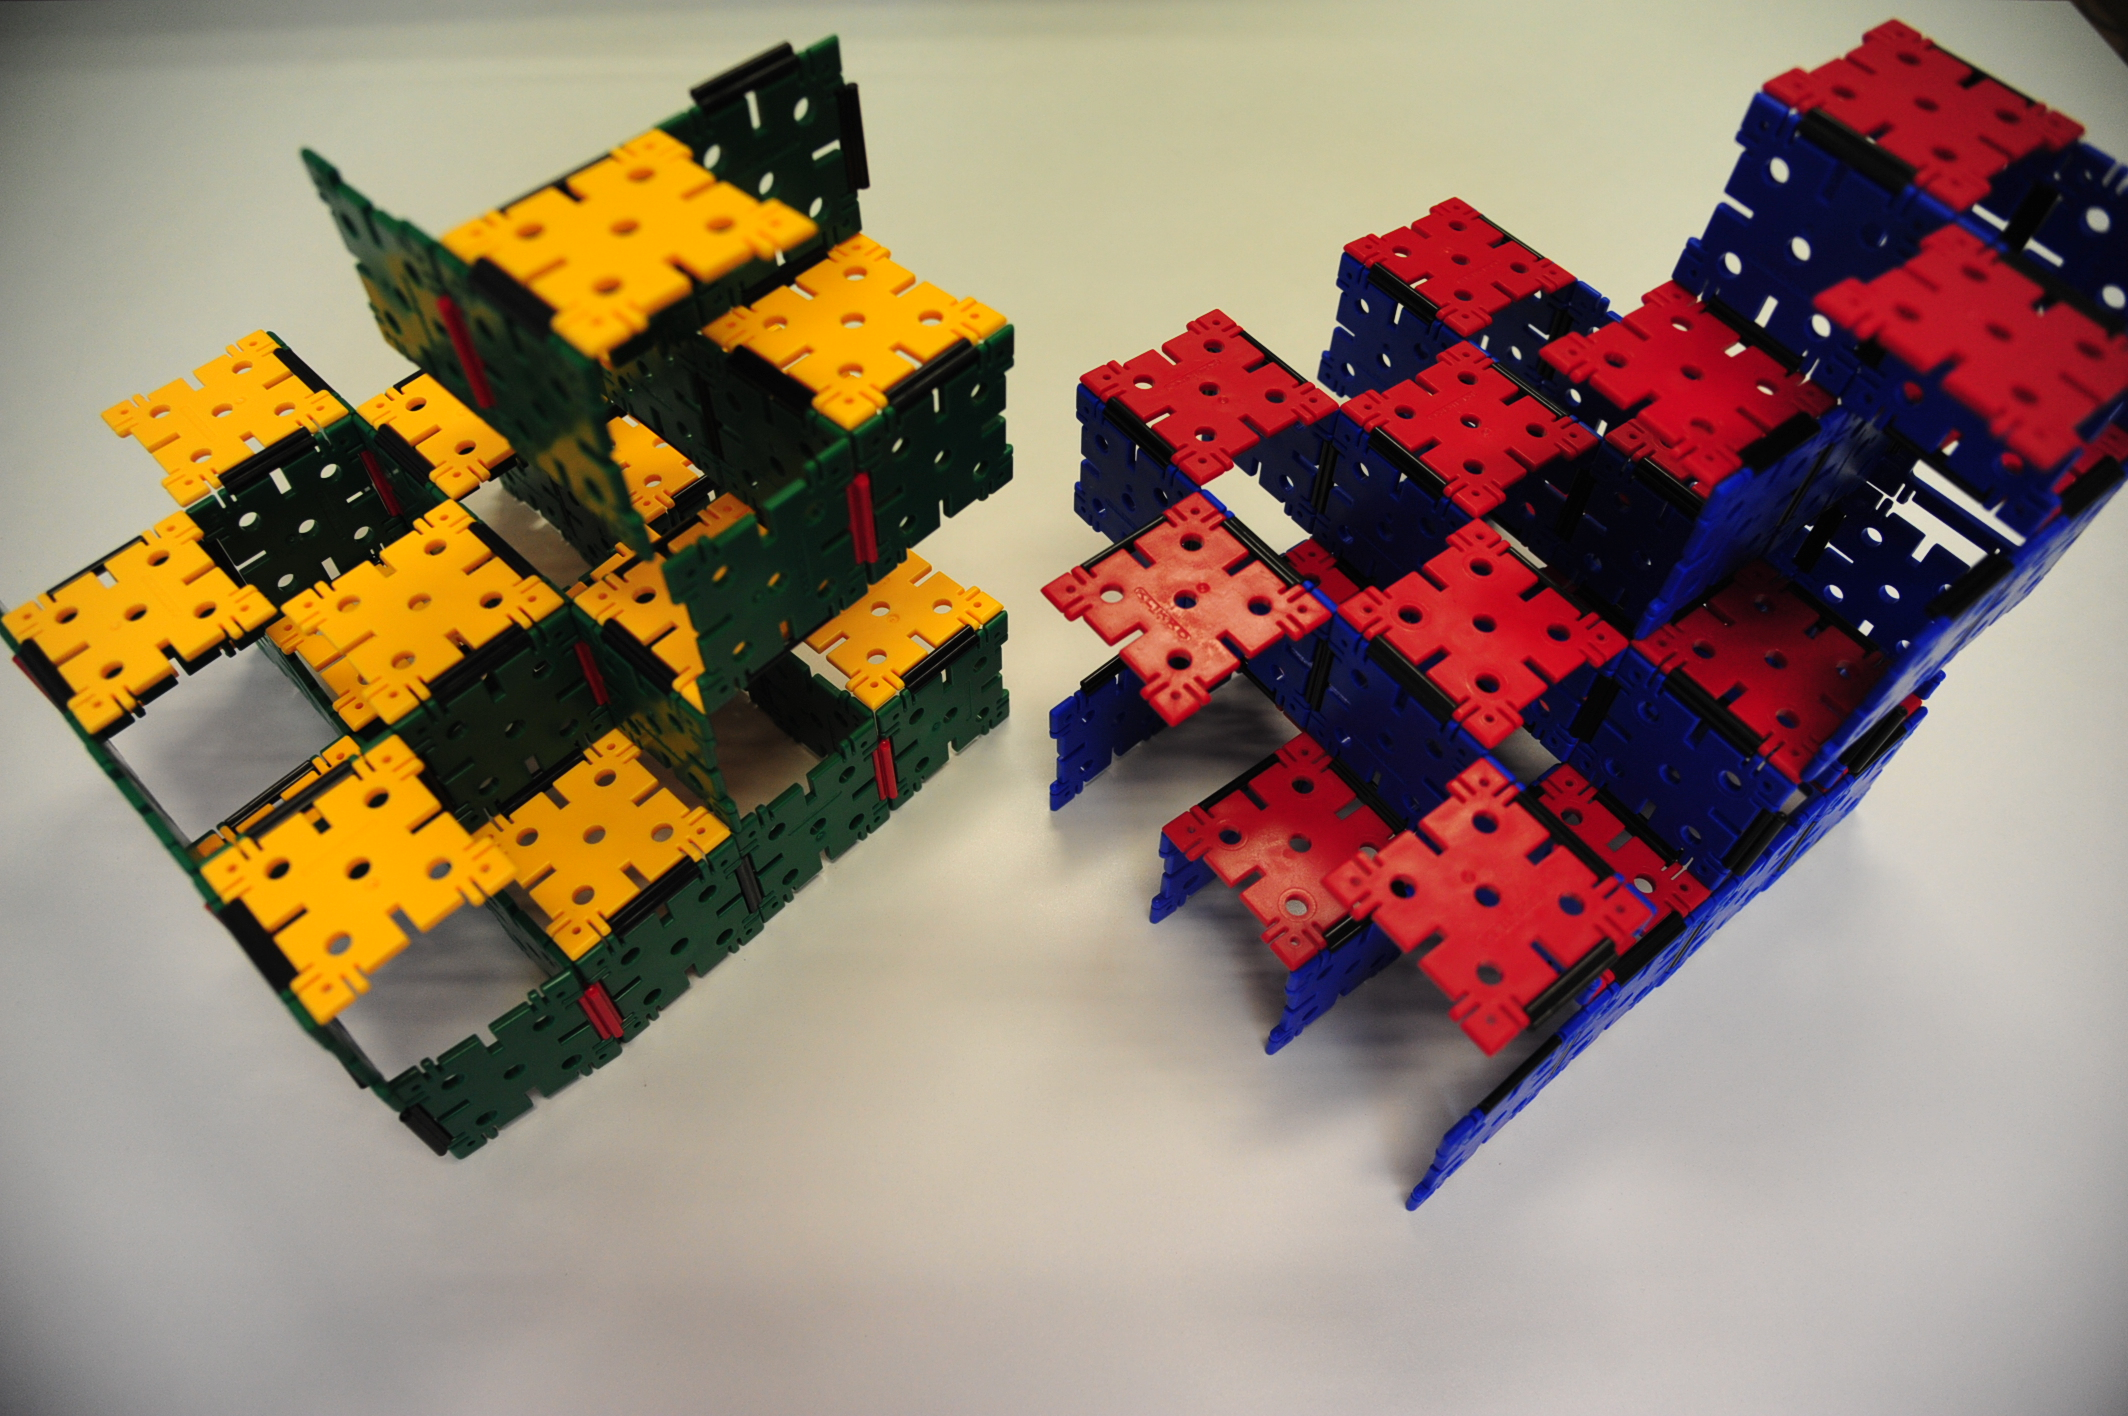
\includegraphics[height=4cm]{toys}
			%\end{center}
  \end{frame}
}


% Delete this, if you do not want the table of contents to pop up at
% the beginning of each subsection:

\begin{document}

\begin{frame}
  \titlepage
\end{frame}

\begin{frame}{Collaborators}
\begin{itemize}
%\item Yunqing Ouyang (欧阳云卿): Fudan University.
%\item Qing-Rui Wang (王晴睿): Chinese University of Hong Kong $\rightarrow$ Yale University.
%\item Zheng-Cheng Gu (顾正澄): Chinese University of Hong Kong.
\item Yunqing Ouyang: Fudan University.
\item Qing-Rui Wang: Chinese University of Hong Kong $\rightarrow$ Yale University.
\item Zheng-Cheng Gu: Chinese University of Hong Kong.
\begin{center}
	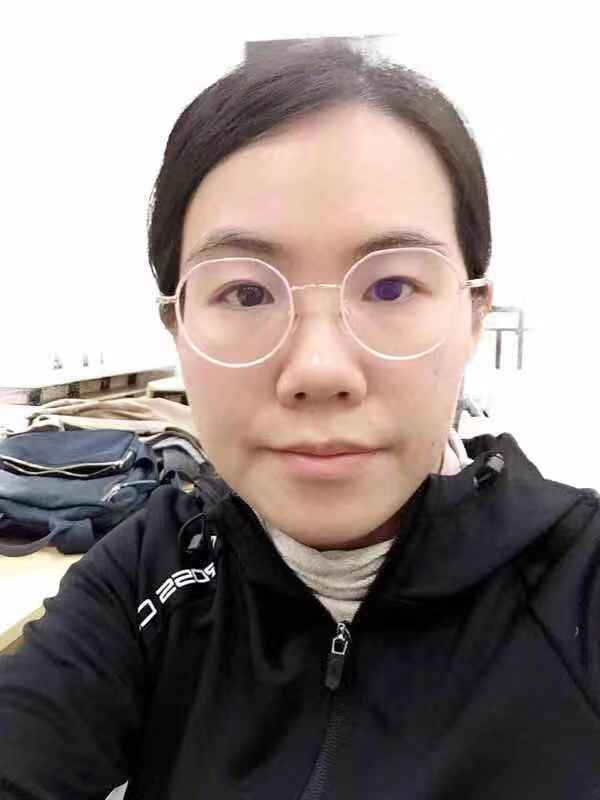
\includegraphics[height=3cm]{../people/yunqing}
	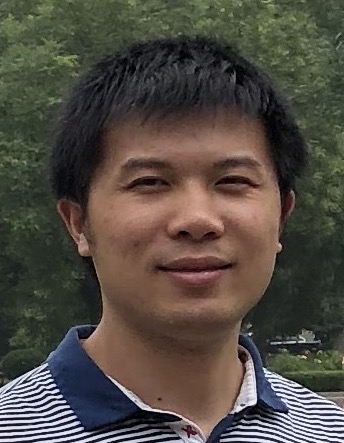
\includegraphics[height=3cm]{../people/qingrui}
	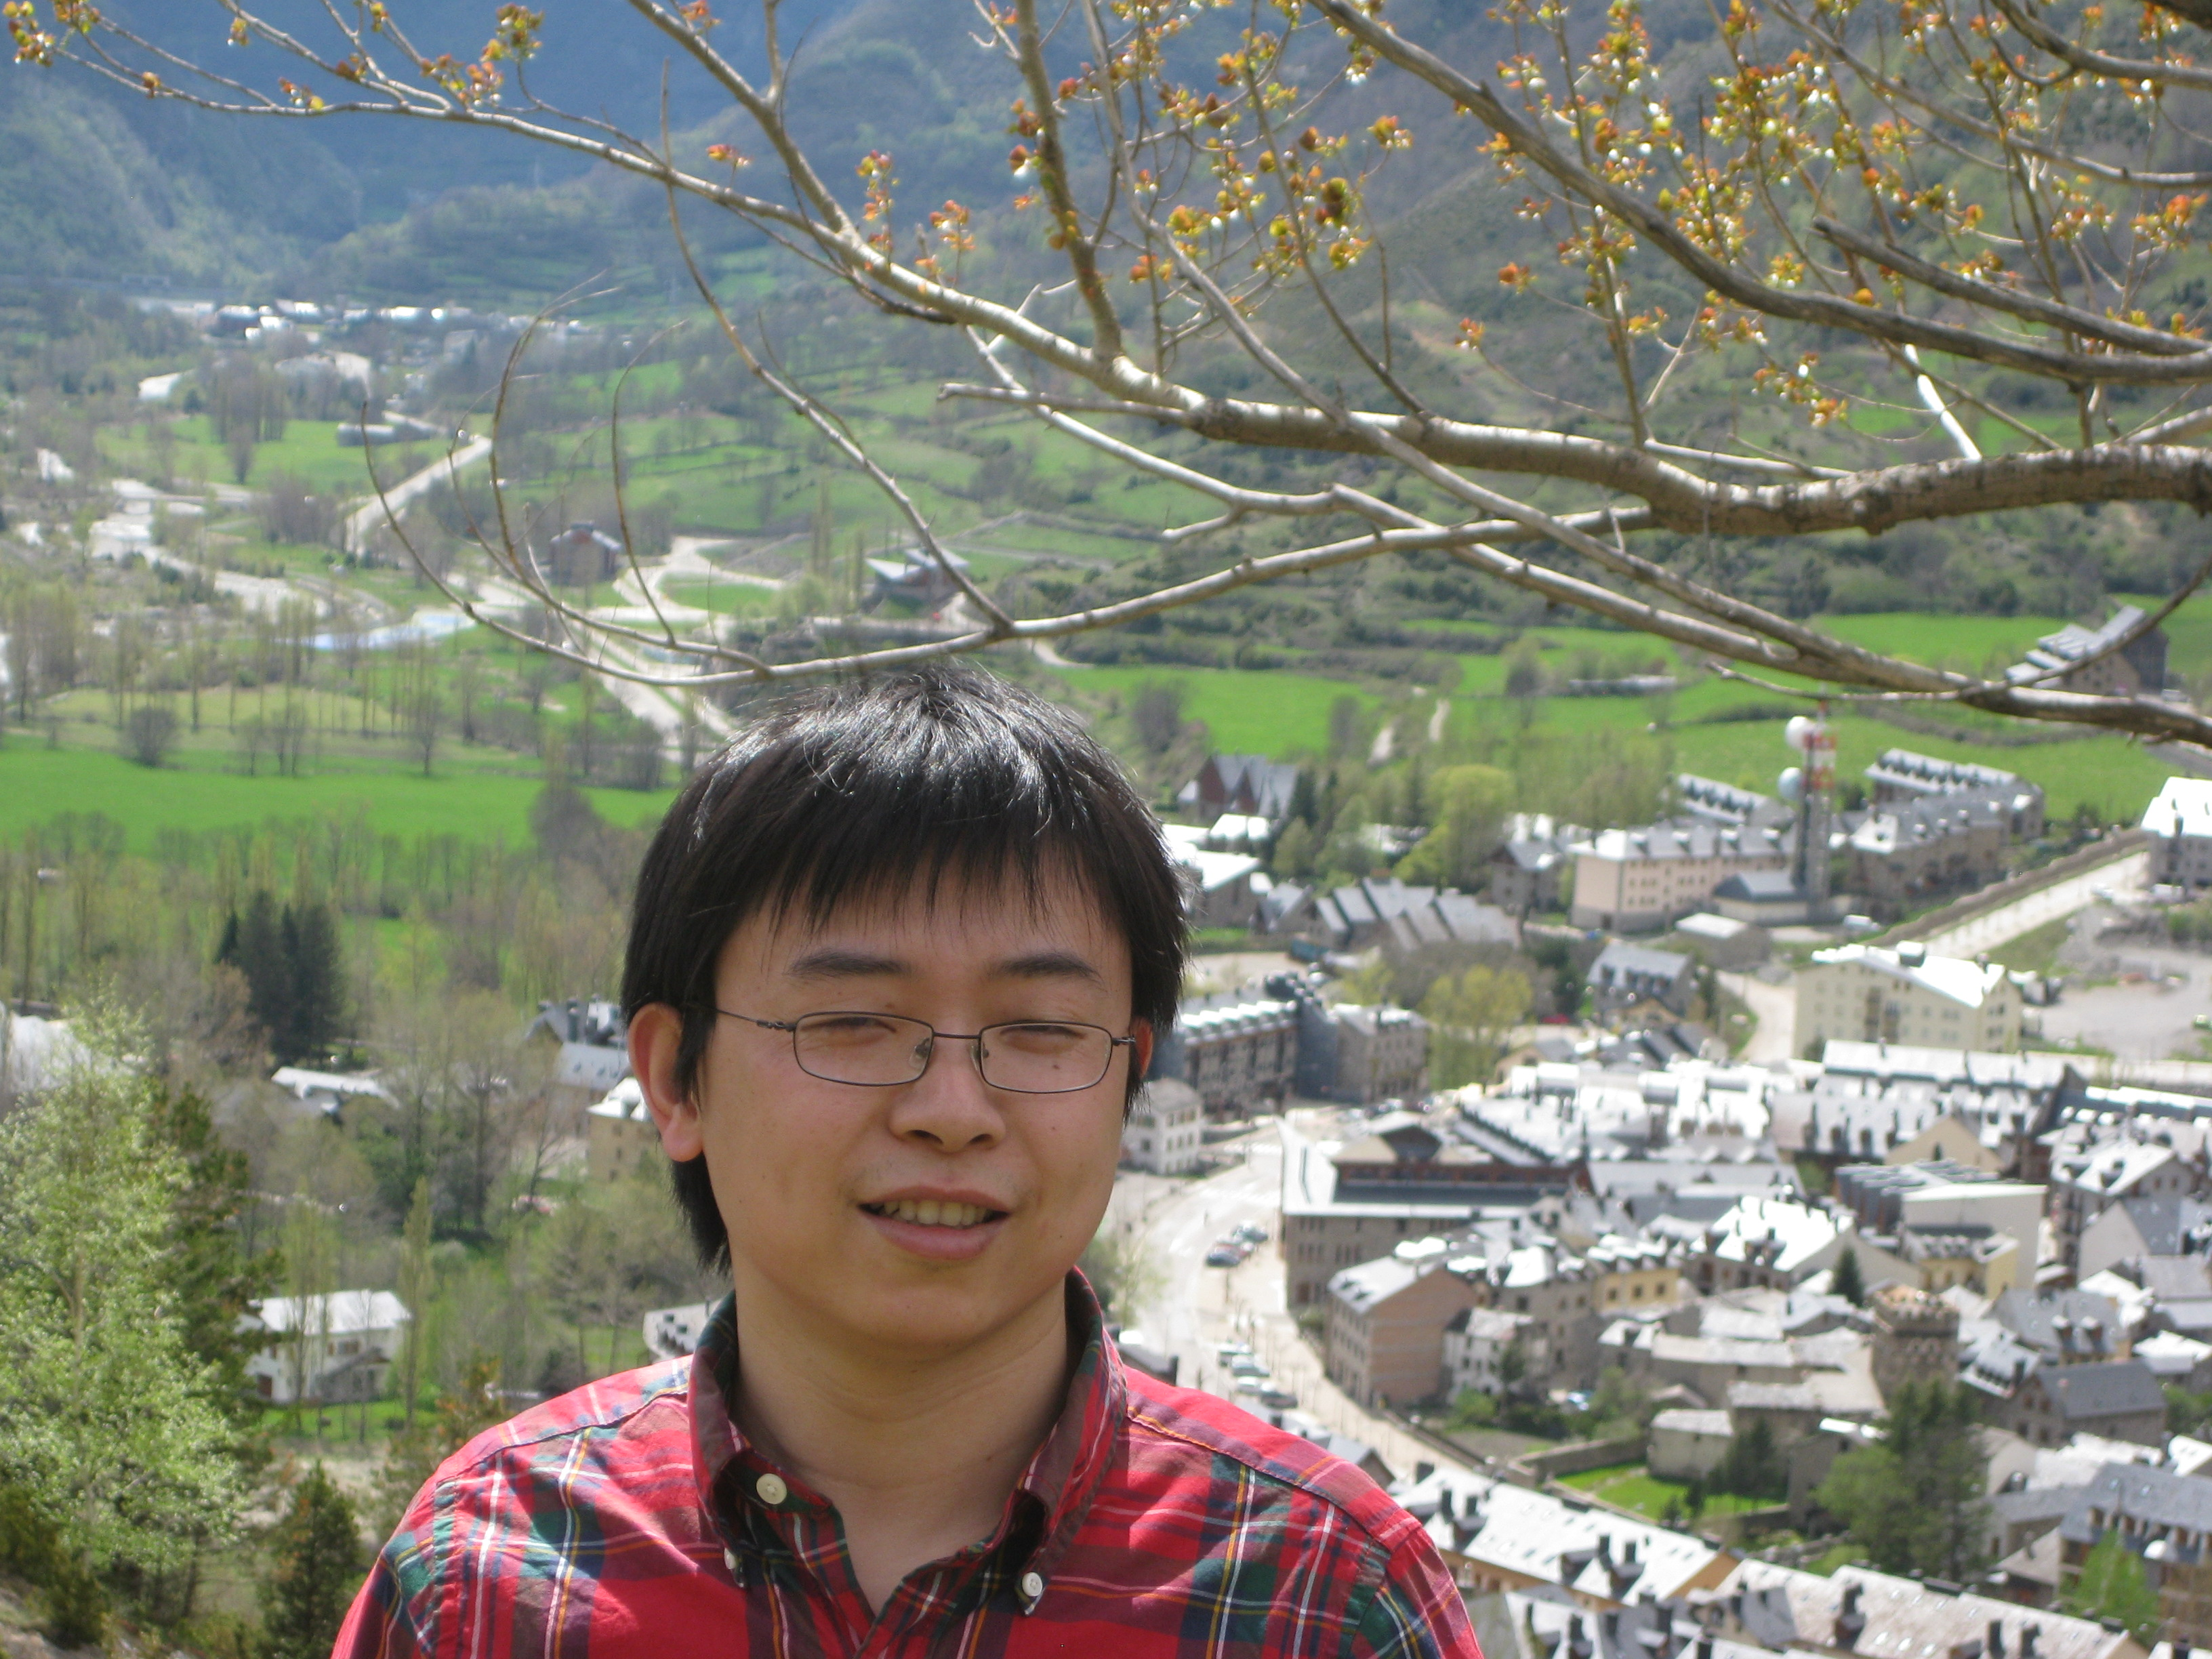
\includegraphics[height=3cm]{../people/zhengcheng}
\end{center}
\item Yunqing Ouyang, Qing-Rui Wang, Zheng-Cheng Gu and YQ, to appear.
\end{itemize}
\end{frame}

\section{Demo: GAP, HAP and SptSet.}

\begin{frame}[fragile]
\frametitle{GAP}
\begin{itemize}
\item GAP = Group, Algorithm and Programming.
\item \url{www.gap-system.org}
\item Easy to create and study groups.
\end{itemize}

\begin{lstlisting}[basicstyle=\footnotesize]
gap> G := CyclicGroup(4);
pc group of size 4 with 2 generators>
gap> G := DihedralGroup(6);
pc group of size 4 with 2 generators>
gap> G := SpaceGroup(3, 105);
SpaceGroupOnRightBBNWZ( 3, 4, 5, 1, 2 )
\end{lstlisting}

\end{frame}

\begin{frame}[fragile]
	\frametitle{HAP and group cohomology}
	\begin{itemize}
		\item bSPT: $H^D[G,\uone]$ can be computed directly using HAP in GAP.
		\item $H^D[G,\uone]$ ``='' $H^{D+1}[G,\mathbb Z]$. \emph{See X-G Wen, PRB \textbf{91}, 205101 (2015)}
	\end{itemize}
	\begin{columns}
		\column{.5\columnwidth}
	\begin{lstlisting}[basicstyle=\footnotesize]
gap> LoadPackage("HAP");
gap> G := CyclicGroup(4);
pc group of size 4 with 2 generators>
gap> GroupCohomology(G, 2);
[ 4 ]
gap> GroupCohomology(G, 3);
[  ]
gap> GroupCohomology(G, 4);
[ 4 ]
gap> GroupCohomology(G, 5);
[  ]
\end{lstlisting}
	\column{.5\columnwidth}
	\[H^{2n+1}[\mathbb Z_4,\uone] = \mathbb Z_4\]
	\[H^{2n}[\mathbb Z_4,\uone] = \mathbb Z_1\]
	\end{columns}
\end{frame}

\begin{frame}[fragile]
	\frametitle{My Package SptSet: computing fSPT and beyond}
	Consider 2D fSPT, $G=\mathbb Z_4$:
\begin{lstlisting}[basicstyle=\footnotesize]
gap> LoadPackage("SptSet");;
gap> G := CyclicGroup(4);;
gap> R := ResolutionFiniteGroup(G, 6);;
gap> utAct := SptSetTrivialGroupAction(G);;
gap> ss := FermionEZSPTSpecSeq(R, utAct);;
gap> FermionSPTLayers(ss, 2);
[ <ZL-Module with torsions [ 2 ]>, <ZL-Module with torsions [ 2 ]>,
  <ZL-Module with torsions [ 4 ]> ]
gap> z2tAct := GroupHomomorphismByImagesNC(G, GL(1, Integers),
>   GeneratorsOfGroup(G), [ [[-1]], [[1]] ]);;
gap> ss := FermionEZSPTSpecSeq(R, z2tAct);;
gap> FermionSPTLayers(ss, 2);
[ <ZL-Module with torsions [ 2 ]>, <ZL-Module []>, <ZL-Module []> ]
\end{lstlisting}

Example: compute fSPT for 2D wallpaper groups.
\end{frame}

\section{Structure: fSPT and general invertible Topological Order classification}

\begin{frame}
  \frametitle{Motivation: bosonic SPT}
  \begin{itemize}
		\item Wave functions are symmetric cochains:
		\[\omega(gg_0,\ldots gg_{d+1})=\rho_T(g)\omega(g_0,\ldots g_{d+1}),\quad
		\omega\in\Psi^d(G) = C^{d+1}[G, \uone_T].\]
		\item Bulk-boundary correspondence:
		\begin{columns}
			\column{.6\textwidth}
			\[d\omega = \nu,\quad d:C^d[G, \uone_T]\rightarrow C^{d+1}[G, \uone_T]\]
			\[d\omega(g_0,\ldots,g_{d+1})
			=\sum_i(-1)^i\omega(g_0,\ldots,\hat g_i,\ldots,g_{d+1}).\]
			\column{.4\textwidth}
			\begin{center}
				\begin{tikzpicture}
				\fill (.5, .5)--(4.5, 0.5)--(5, 1)--(5, 2)--(1, 2)--(0.5, 1.5)--(0.5, 0.5) [mbg!15];
				\node at (2.75, 1.5) {$\nu$};
				\fill (0.5, 0.5)--(4.5, 0.5)--(5, 1)--(1, 1)--(0.5, 0.5) [mbg];
				\node  [text=white] at (2.75, 0.75) {$\omega$};
				\draw (1, 1)--(1, 2) [black!40];
				\draw (0.5, 0.5)--(0.5, 1.5) [black!40];
				\draw (5, 1)--(5, 2) [black!40];
				\end{tikzpicture}
			\end{center}
		\end{columns}
  \item A cochain complex and its cohomology group:
	\[\Psi^0(G)\xrightarrow{d^0}\Psi^1(G)
	\xrightarrow{d^1}\Psi^2(G)
	\xrightarrow{d^2}\Psi^3(G)
	\xrightarrow{d^3}\Psi^4(G)
	\xrightarrow{d^4}\Psi^5(G)
	\rightarrow\cdots\]
\[\Phi^d(G) = H^{d+1}[G,\uone_T]=\{d\omega=0\}/\{\omega\simeq\omega+d\mu\}=\frac{\ker d}{\img d}.\]
  \end{itemize}
\end{frame}

\begin{frame}
	\frametitle{Fixed-point anomalous states / wave functions}
	\begin{itemize}
		\item State space: $\Psi^d(G)$. (Including \alert{anomalous} SPT states.)
		\item Stacking operation: $\psi_1\boxplus\psi_2$.
		Could be non-Abelian: $\psi_1\boxplus\psi_2\neq\psi_2\boxplus\psi_1$.
		\item Coboundary operation: $\delta:\Psi^d(G)\rightarrow\Psi^{d+1}(G)$;\\
		$\delta\alpha=\beta$ means $\alpha$ is realized on the surface of $\beta$.
		\item $\delta(\psi_1\boxplus\psi_2)=\delta\psi_1\boxplus\delta\psi_2$.
		\item $\psi_1\boxplus\psi_2-\psi_2\boxplus\psi_1\in \delta(\Psi^{d-1}(G))$.
		\item A cochain complex and its cohomology group:
		\[\Psi^0(G)\xrightarrow{\delta^0}\Psi^1(G)
		\xrightarrow{\delta^1}\Psi^2(G)
		\xrightarrow{\delta^2}\Psi^3(G)
		\xrightarrow{\delta^3}\Psi^4(G)
		\xrightarrow{\delta^4}\Psi^5(G)
		\rightarrow\cdots\]
	\[\Phi^d(G) =\frac{\delta\alpha=0}{\alpha\sim\alpha+\delta\beta}=\frac{\ker \delta^d}{\img \delta^{d-1}}.\]
	\end{itemize}
\end{frame}

\begin{frame}
	\frametitle{Fermionic SPT states}
	\begin{itemize}
		\item $\Psi^d(G)=C^0(G_b, \Omega^{d+1})\times C^1(G_b, \Omega^d)\times\cdots\times
	  C^{d+1}(G_b, \Omega^0)$, $G_b=G/\mathbb Z_2^f$.
		\item $C^p$: decoration on codimension-$p$ domain walls.
		\item $\Omega^q$: $q$-dimensional invertible topological order.
		\[\Omega^0=\uone_T,\quad\Omega^1=\mathbb Z_2,\quad\Omega^2=\mathbb Z_2,\quad\Omega^3=\mathbb Z_T.\]
		\item $\psi\in \Psi^d(G)$: $\psi=\begin{pmatrix}\psi^0&\psi^1&\cdots&\psi^{d+1}\end{pmatrix}$.
	\end{itemize}
	\begin{center}
		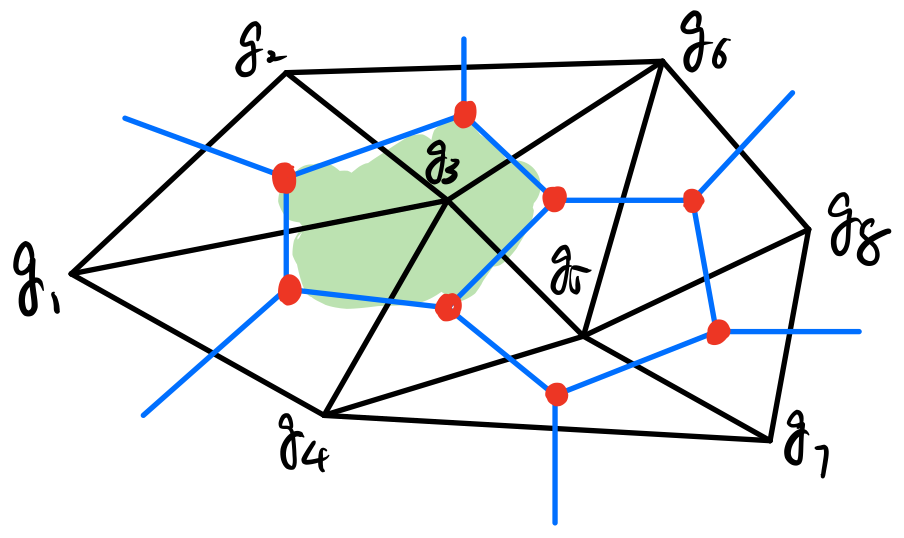
\includegraphics[height=3cm]{decoration}
	\end{center}
\end{frame}

\begin{frame}
	\frametitle{Stacking operation}
	\begin{itemize}
		\item Not a simple component-wise addition:
		$\psi_1\boxplus\psi_2\neq (\psi_1^{d+1}+\psi_2^{d+1},\ldots,\psi_1^0+\psi_2^0)$.
		\item Reason: reordering of fermionic degrees of freedom.
		\item Result on the $p$-th layer will be twisted by higher layers.
		\[(\psi_1\boxplus\psi_2)^p = \psi_1^p + \psi_2^p
    + \mathcal A^{p,d-p+1}(\psi_1^{d+1},\psi_2^{d+1},\ldots,\psi_1^{p+1}, \psi_2^{p+1}),\]
		\item Examples: in 2d, $G=G_b\times\mathbb Z_2^f$
		\begin{align*}
		  \mathcal A^{21} &= \psi^1_1\cup\psi^1_2;\\
		  \mathcal A^{30} &= \frac12\psi^2_1\cup_1\psi^2_2 + \frac12 (\psi^1_1\cup\psi^1_2)\cup_1(\psi^2_1+\psi^2_2).
		\end{align*}
	\end{itemize}
	\begin{center}
		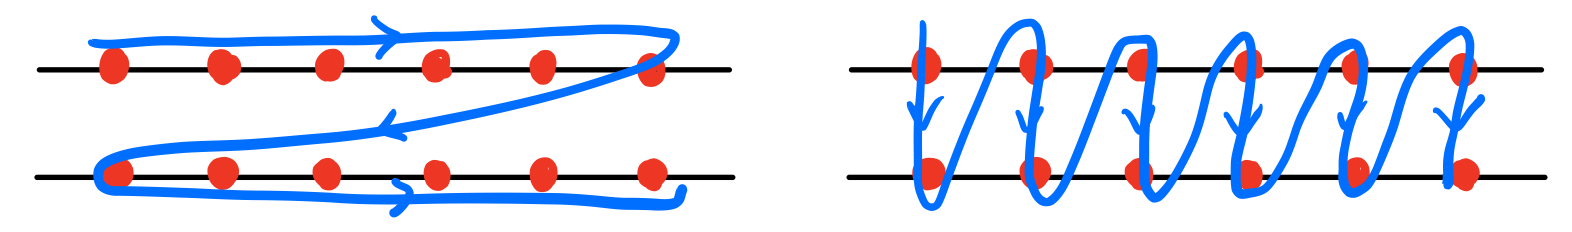
\includegraphics[height=2cm]{forder}
	\end{center}
\end{frame}

\begin{frame}
	\frametitle{Coboundary operation}
	\begin{itemize}
		\item Consider the coboundary of a single-layer state
		$\psi = \begin{pmatrix}0&\cdots&\psi^p&\cdots&0\end{pmatrix}$.
		\item $\delta\psi$ only contains layers $p'<p$:
		$\delta\psi=\begin{pmatrix}0&\cdots&d\psi^p&(\delta\psi)^{p+2}\cdots&(\delta\psi)^{d+2}\end{pmatrix}$.
		\item We denote $(\delta\psi)^{p'}=\mathcal D^{p, d-p+1}_{p'-p}(\psi^p)$.
		$D^{pq}_r:C^p(G_b,\Omega^q)\rightarrow C^{p+r}(G_b,\Omega^{q-r+1})$.
		\item $d$ is like an upper-triangular matrix.
		\item Examples: in 2d, $G=G_b\times\mathbb Z_2^f$
		\begin{align*}
			\mathcal D_2^{12} &= s\cup\psi^1\cup\psi^1,\\
		  \mathcal D_2^{21} &= \frac12\psi^2\cup\psi^2
		  +\frac12\psi^2\cup_1d\psi^2
		  +\mathcal O_4'(d\psi^2).
		\end{align*}
		\[  O_4'(\psi^2)(01234)
		  =\frac12d\psi^2(0124)d\psi^2(0234)
		  -\frac14\{d\psi^2(0123)[1-d\psi^2(0124)] \mod 2\}.\]
	\end{itemize}
\end{frame}

\begin{frame}[fragile]
	\frametitle{Input formulas into the SptSet package}
	\begin{itemize}
		\item The functions $\mathcal A^{pq}$ and $\mathcal D^{pq}_r$ needs to be inputed.
		\item Example: $\mathcal D_2^{12} = s\cup\psi^1\cup\psi^1$.
	\end{itemize}

	\begin{block}{GAP realization}
	\begin{lstlisting}[basicstyle=\footnotesize,morekeywords={function,return,local,if,fi,then,end},showspaces=false,showtabs=false, keywordstyle=\color{blue}]
	SptSetInstallCoboundary(ss, 2, 1, 2,
	function(n1, dn1)
		return {g1, g2, g3} -> (s(g1) * n1(g2) * n1(g3));
	end);
	\end{lstlisting}
	\end{block}

\end{frame}

\section{Algorithm: there is a spectral sequence}

\begin{frame}
	\frametitle{There is a spectral sequence...}
	\begin{itemize}
		\item Atiyah–Hirzebruch Spectral Sequence:
		b/c $d$ is upper triangular.
		\[E^{pq}_2=H^p(G_b,\Omega^q)\Rightarrow \Phi^{p+q-1}(G).\]
		\item Spectral sequence is like a perturbation theory.
		\item $E^{pq}_\infty$: $(p+q-1)$-d SPT phases represented by
		$\begin{pmatrix}0&\cdots&0&\psi^p&\psi^{p+1}&\cdots\end{pmatrix}$.
		\item $E^{pq}_r$: $r^{th}$-page approximation.
		\item $r^{th}$-page boundary-bulk correspondence:\\
		$\delta\alpha\simeq\beta$ mod $(p+r+1)$-layer and higher layers.
		\begin{enumerate}
			\item $r=1$: $(\delta\alpha)^p = d\alpha^p = \beta^p$.
			\item $r=2$: $(\delta\alpha)^{p+1} = \mathcal D^{pq}_2(\alpha^p) + d\alpha^{p+1} = \beta^{p+1}$
			\item $r=3$: $(\delta\alpha)^{p+2} = \mathcal D^{pq}_3(\alpha^p)
			 + \mathcal D^{p+1,q}_2(\alpha^{p+1}) + d\alpha^{p+2} = \beta^{p+2}$
			\item $\cdots$.
		\end{enumerate}
	\end{itemize}
\end{frame}

\begin{frame}
	\frametitle{$r^{th}$-page derivative}
	\begin{itemize}
		\item $d_r: E^{pq}_r\rightarrow E^{p+r,q-r+1}_r$.
		\item $d_r: \alpha\mapsto\beta$, s. t.
		\begin{enumerate}
			\item $\delta\alpha\simeq0 \mod (r-1)$, or $(\delta\alpha)^p=\cdots=(\delta\alpha)^{p+r-1}=0$
			\item $\delta\alpha\simeq\beta\mod r$, or $\beta^{p+r}=(\delta\alpha)^{p+r}$
		\end{enumerate}
		\item Examples:
		\begin{enumerate}
			\item $E^{pq}_1=C^p(G_b, \Omega^q)$.
			\item $d_1: \alpha\mapsto(\delta\alpha)^p=d\alpha^p$.
			\item $d_2:$ $d\alpha^p=0$; $\alpha\mapsto(\delta\alpha)^{p+1}=\mathcal D_2^{pq}(\alpha^p)+d\alpha^{p+1}\simeq D_2^{pq}(\alpha^p)$.
			\item $d_3$: $d\alpha^p=0,d\alpha^{p+1}=-\mathcal D_2^{pq}(\alpha^p)$;
			$\alpha\mapsto(\delta)^{p+2}
			=\mathcal D^{pq}_3(\alpha^p)
			 + \mathcal D^{p+1,q}_2(\alpha^{p+1}) + d\alpha^{p+2}
			\simeq\mathcal D^{pq}_3(\alpha^p)
			 + \mathcal D^{p+1,q}_2(\alpha^{p+1})$.
		\end{enumerate}
		\item Bulk-boundary corresdpondence: $d_r\alpha = \beta$ implies
		\begin{enumerate}
			\item Cocycle condition: $d_r\alpha=0$.
			\item Coboundary equivalence: $\alpha\sim\alpha+d_r\beta$.
		\end{enumerate}
		\item Iterative calculation:
		$E^{pq}_r=\frac{\ker d_r^{pq}}{\img d_r^{p-r,q+r-1}}$.
	\end{itemize}
\end{frame}

\begin{frame}
	\frametitle{Advantage of using spectral sequence}
	\begin{itemize}
		\item Naively: checking all cocycle conditions $d_r\alpha=0$, and mod out all coboundary equivalences $\alpha\simeq\alpha+d_r\beta$.
		\item Using SS:
		\begin{enumerate}
			\item $d_2\alpha=0$ / $\alpha\simeq\alpha+d_2\beta$;
			\item $d_3\alpha=0$ / $\alpha\simeq\alpha+d_3\beta$;
			\item $\cdots$.
		\end{enumerate}
		\item Advantage of doing cocycle/coboundary in a synchronized way:
		Consider the example of $d_3$.
		\begin{itemize}
			\item $d_3:E^{pq}_3\rightarrow \alert{E^{p+3, q-2}_3}$.
			\item Take $\alpha\in E^{pq}_3$, choose $\alpha^{p+1}$ such that $d\alpha^{p+1}=-\mathcal D_2^{pq}(\alpha^p)$.
			\item $d_3\alpha\simeq\mathcal D^{pq}_3(\alpha^p)
			 + \mathcal D^{p+1,q}_2(\alpha^{p+1})$.
			 \item \alert{Only need to examine a special solution} of $\alpha^{p+1}$:\\
			 If we choose another solution $\tilde\alpha^{p+1}=\alpha^{p+1}+\beta^{p+1}$,\\
			 $d_3\alpha\simeq\mathcal D^{pq}_3(\alpha^p)
 			 + \mathcal D^{p+1,q}_2(\alpha^{p+1})+\alert{\mathcal D^{p+1,q}_2(\beta^{p+1})}\simeq D^{pq}_3(\alpha^p)
 			 + \mathcal D^{p+1,q}_2(\alpha^{p+1})$.
			 \item $\mathcal D^{p+1,q}_2(\beta^{p+1})\in\img d_2^{p+1,q-1}$ was mod out when computing $E^{p+3,q-2}_3$,
		\end{itemize}
	\end{itemize}
\end{frame}

\section{Algorithm: simplified resolution and chain maps}

\begin{frame}
	\frametitle{Simplified resolution and chain maps}
	\begin{itemize}
		\item A problem: cochains $\alpha(g_0,\ldots,g_n)$ are too complicated to deal with.
		\item A simplified resolution: a simplified basis replacing $[g_0,\ldots,g_n]$.
		\item Chain maps: a ``compiler'' converting formulas from the standard basis to the simplified basis.
		\item Allows computation for infinite (discrete) groups.
	\end{itemize}
\end{frame}

\section{Summary}

\begin{frame}
	\frametitle{Summary}
	\begin{itemize}
		\item Use a spectral sequence to compute fSPT classification.
		\item Use a simplified free resolution to accelerate computation of group cohomology.
		\item We are working on a GAP package SptSet.
		\item Takes 5min to compute 2D fSPTs for all 17 wallpaper groups.
		\item Email me at \url{qiyang@fudan.edu.cn} for early access.
		\item We also have a program written in python: faster but much harder to use.
		\item Will add more functions (fSPT with nontrivial group extension, group structure, ...), tweak the performence, and publish.
	\end{itemize}
\end{frame}

\end{document}
